
\documentclass{article}
\usepackage{graphicx}
\usepackage{float}
\usepackage[utf8]{inputenc}
\title{Report: Equipment Demonstration}
\author{Cole Rottenberg \\ 11062528}
\date{\today}

\begin{document}

\maketitle

\section*{Introduction}
    The topic of this lab is to familiarize ourselves with the equipment we will be using throughout the semester. This includes the oscilloscope, multimeter, power supply, and function generator. We will also be using the lab equipment for the rest of our design classes. 
These tool allow us to collect data and debug our physical hardware more effectively. In addition, the programmability of the power supply, function generator, and scope allow us to automate the testing process. This allows us to test our hardware more efficiently and accurately.
% Add your introduction content here
\section*{Design}
    \subsection*{Report}
    \begin{enumerate}
       \item A div is a measurement of the distance between two vertical or horizontal lines on the screen. Adjustment for visaul purpose can modulate time and voltage per div to allow for better viewing of the signal. 
       \item With one set of the power supply leads, we can set the voltage to +- 12V. The other set limited to 5V, we can set to 0V and 5V.
       \item 
       \begin{enumerate}
        \item With a programmable power supply, we can detect faulty components by setting the voltage to a certain level and plotting the current. As faulty components get hot, there will be a drop in current as the resistance increases.
        \item Using the oscilloscope, we can debug the DAC over SPI using the logic analyzer built-in to not only read the data being sent, but also the clock and chip select lines.
       \end{enumerate}
       \item Using the multimeter, we can test the current and voltage to the microcontroller to ensure it is getting the correct power.
       \item
       \begin{enumerate}
        \item Using a 220k$\Omega$ resistor and a 1nF capacitor, we can create a low pass filter to filter out the noise from the signal. The theoretical cutoff frequency is \textbf{723.43 Hz}.     
        \item 
        \begin{figure}[H]
            \centering
            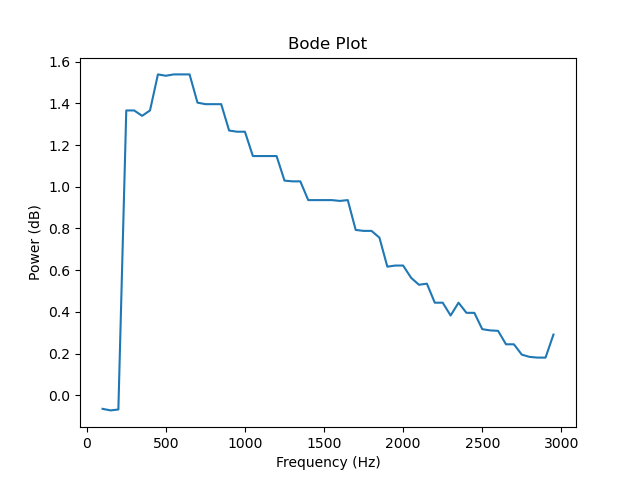
\includegraphics[width=1\textwidth]{bode.png}
            \caption{Low Pass Filter}
            \label{fig:filter}
        \end{figure}
        \item The actual resistance is 217.5k$\Omega$ and the actual capacitance is 1.1nF. The actual cutoff frequency is \textbf{666.7 Hz}. The new caluclaution for the cutoff frequency matches the bode plot more accurately.
       \end{enumerate}
    \end{enumerate}

% Add your design content here

\section*{Conclusion}
The final testing our of resistor and capacitor further highlight how even with a 5\% tolerance, the actual values can be far off from the theoretical values. This is why it is important to test the components before using them in a circuit.
\end{document}
